\scanpage{21}
\mspage{20}
\mspage{IV-\unsure{952}}

\uline{neau} $({}^h A)_{\underline p}/\underline p\cdot({}^h A)_{\underline p}$ \uline{est} \deleted{\unsure{produit}} \uline{composé direct d'un nombre fini d'extensions algébriques séparables de} $\kappa(\underline p)$ (ce qui entraîne que les fibres du morphisme canonique $\operatorname{Spec}({}^h A)\to\operatorname{Spec}(A)$ sont \uline{géométriquement régulières}).

(i) Comme ${}^h A$ est un $A$-module fidèlement plat, il résulte de (2.1.13) que si ${}^h A$ est \deleted{\unsure{un}} réduit (resp. normal), il en est de même de $A$. Pour prouver la réciproque, on peut se borner au cas où l'anneau $A$ est local, de sorte \deleted{\unsure{à}} qu'avec les notations de (18.6.4), on a ${}^h A=\varinjlim A_\alpha$. Or, il résulte de la définition des $A_\alpha$ et de (17.5.7) que si $A$ est réduit (resp. intègre et intégralement clos), il en est de même des $A_\alpha$ ; \deleted{\unsure{en}} en outre, les \deleted{\illegible{2}} \deleted{\illegible{7}} morphismes \deleted{$\operatorname{Spec}(A_\beta)\to\operatorname{Spec}(A_\alpha)$} \inserted{$A_\alpha\to A_\beta$} pour $\alpha\leq\beta$ sont \deleted{surjectifs} \inserted{injectifs} en vertu de \deleted{(2.5.4,(ii))}. On conclut donc de (5.13.2) (resp (5.13.4)) que ${}^h A$ est réduit (resp. intègre et intégralement clos).
\margin{\unsure{précieux|curieux} \unsure{mélange !}}

(ii) \inserted{On peut se borner au cas où $A$ est local.} En vertu du fait que le foncteur $\varinjlim$ permute au produit tensoriel, la fibre du morphisme $\operatorname{Spec}({}^h A)\to\operatorname{Spec}(A)$ en un point $p$ est limite inductive des fibres des morphismes $\operatorname{Spec}(A_\alpha)\to\operatorname{Spec}(A)$ en ce point. . Comme ${}^h A$ est noethérien, on voit, compte tenu de (17.6.2), que l'on est ramené à prouver le lemme suivant :

\uline{Lemme} (18.6.9.1).-- \uline{Soient} \deleted{$\unsure{B}$} $(B_\alpha)$ \uline{un système inductif d'anneaux artiniens}, $B=\varinjlim B_\alpha$ \uline{sa limite inductive. Si} $B$ \uline{est noethérien, alors} $B$ \uline{est artinien} ; \deleted{\illegible{9}} \uline{si de plus, pour} $\alpha\leq\beta$, \uline{les homomorphismes} \inserted{$\varphi_{\beta\alpha}:$} $B_\alpha\to B_\beta$ \uline{sont injectifs, alors il existe} $\lambda$ \uline{tel que, pour} $\alpha\geq\lambda$ \uline{le nombre des composants locaux} \deleted{\unsure{de}} $B_\alpha^{(\unsure{1|i})}$ \uline{de} $B_\alpha$ \uline{soit constant}, \deleted{\unsure{de sorte}} \uline{que} $\varphi_{\beta\alpha}(B_\alpha^{(\unsure{1|i})})\subset B_\beta^{(\unsure{1|i})}$ \uline{pour tout} $\unsure{1|i}$ \uline{et que les} $B^{(\unsure{1|i})}=\varinjlim B_\alpha^{(\unsure{1|i})}$ \uline{soient les composants locaux de} $B$.

Soient en effet $Y_\alpha=\operatorname{Spec}(B_\alpha)$, $Y=\operatorname{Spec}(B)$, qui, en tant qu'espace topologique, est égal à $\varprojlim Y_\alpha$ (8.2.10). Les espaces $Y$ étant \deleted{\unsure{compacts}} \inserted{finis et} discrets, la seconde assertion du lemme résultera de la première et du fait que si les $\varphi_{\beta\alpha}$ sont injectifs, les morphismes canoniques $Y_\beta\to Y_\alpha$ sont surjectifs. On est ainsi ramené à prouver le lemme purement topologique suivant :
\margin{\unsure{peu clair}}
\margin{\figure{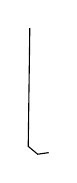
\begin{tikzpicture}[x=1cm,y=1cm]\draw (0,1.6)--(-.02,.1)--(.1,0)--(.24,.02);\end{tikzpicture}}}

\uline{Lemme} (18.6.9.2).-- \uline{Soit} $(Y_\alpha)$ \uline{un système projectif d'espaces topologiques finis et discrets. Si} $Y=\varprojlim Y_\alpha$ \uline{est noethérien}, $Y$ \uline{est fini et discret}.

